%%==================================================
%% chapter01.tex for BIT Master Thesis
%% modified by yang yating
%% version: 0.1
%% last update: Dec 25th, 2016
%%==================================================
% \chapter{基于分类器自适应知识蒸馏的事件检测框架}
\chapter{基于分类器自适应知识蒸馏的数据不平衡依赖消解}
\label{chap:chapter3}

事件检测作为事件抽取的基础子任务,其数据集中存在严重的数据不平衡现象,限制了不同事件检测模型系统的事件识别能力。针对该问题,现有方法主要利用人工设计的损失函数减少不平衡数据产生的负面影响。然而,这些方法特定于具体的模型架构和任务设计,依赖额外超参数,阻碍了其在不同数据不平衡情况下的扩展应用。为此,本章提出了一种基于分类器自适应知识蒸馏方法,以消解数据不平衡依赖问题。实验结果证明,该方法可以通用有效地提升不同事件检测模型的性能。此外,经本章实验验证,该方法可有效迁移到其他存在数据不平衡依赖的信息抽取任务中,如关系抽取等,证明了其良好的任务普适性。

\section{引言}
随着神经网络技术的快速发展,现有事件检测方法的性能取得了显著提升。然而,事件检测数据集中不存在事件的句子过多,导致这些方法普遍遭受数据不平衡依赖的困扰。例如,在ACE2005数据集的训练集部分,超过76\%的句子文本不存在事件,由此产生的过量负实例(非事件触发词)限制了现有方法高效捕捉正实例(事件触发词)的特性,使得这些方法在识别事件时性能表现有待提升。为了消解此种依赖,一些研究工作致力于增强对于正实例特性的建模或减少过高的负实例比例产生的负面影响。例如,Dos等人~\cite{dos2015classifying}在训练中不使用负实例数据,并利用成对排序损失捕捉正实例的通用特性。Chen等人~\cite{chen2018collective}在事件检测的训练损失中引入偏置参数,使得正实例和负实例以不同的权重进行训练。Ye等人~\cite{ye2019exploiting}提出了一个多任务框架,通过增加一个额外的加权损失函数进行正负实例识别能力的学习,进而更好地捕捉正实例的特性。然而,这些方法依赖于人工设计的损失函数,其需要额外的超参数以适应不同数据集的不平衡程度差异,缺乏可扩展性。此外,这些方法只针对特定的模型架构和任务设计,缺乏通用性。因此,本章研究通用的事件检测框架,在不依赖额外超参数的情况下,自动消解数据不平衡问题。

与现有工作聚焦于调整正实例或负实例的训练权重不同,本章基于数据不平衡依赖问题影响事件检测性能的方式,研究减轻其性能影响的通用方法。根据Ye等人~\cite{ye2019exploiting}的研究工作,可知数据不平衡依赖导致现有模型易将正实例预测为负实例,反之亦然。因此,数据不平衡依赖限制了现有模型识别正负实例的能力,进而降低了整体事件检测性能。

为了提升正负实例的识别性能,本章首先定义了句子级别识别信息,其表示给定实例的所在句子中是否存在事件。例如,给定文本“Mary \underline{died} on Thursday in Memphis.”和实例“died”,已知“died”触发了$Die$事件,则其句子级别识别信息为在该句子中存在事件。若给定文本“Mary lives in Memphis.”和实例“lives”,已知其文本中不存在任何事件触发词,则其句子级别识别信息为在该句子中不存在事件。基于此,在事件检测中引入了该信息,并通过预实验评估了其在消解数据不平衡依赖导致的性能下降方面的优势。表\ref{tab:gap_event}具体展示了在不同事件检测基线模型\footnote{DMRoBERTa为本章结合DMBERT和RoBERTa~\cite{liu2019roberta}而提出的一个变体模型。}中引入句子级别识别信息后的性能变化,其中“TI”和“TC”分别表示事件触发词(正例)识别\footnote{事件触发词识别在表述上等同于事件识别。}和事件检测的F1性能指标,“TI+”和“TC+”分别表示在模型输入中引入句子级别识别信息后对应的“TI”和“TC”。可以观察到,该信息的引入使得不同事件检测基线模型的事件触发词识别性能均显著提升,且提升的识别性能进一步增强其在事件检测任务的整体性能。然而,句子级别识别信息需要根据标注的事件检测标签转化得到,因此无法在推理测试阶段进行利用。

\begin{table}[htp]
\centering
\caption{ACE2005数据集上引入句子级别识别信息在F1(\%)指标上的结果对比}
\begin{tabular}{l|cccc}
\toprule
模型  & TI   & TI+  & TC   & TC+  \\ \midrule
Bi-LSTM~\cite{hochreiter1997long} & 70.1 & 78.6 & 67.8 & 71.7 \\
JMEE~\cite{liu2018jointly}    & 75.2 & 79.4 & 72.8 & 75.4 \\
MOGANED~\cite{yan2019event} & 75.9 & 79.8 & 73.4 & 76.6 \\
% EE-GCN~\cite{cui2020edge} & 78.3 & 81.8 & 77.6 & 79.2 \\
DMBERT~\cite{wang2019adversarial} & 79.4 & 84.4 & 74.6 & 80.0 \\ 
DMRoBERTa & 80.1 & 85.5 & 75.5 & 81.9 \\ \bottomrule
\end{tabular}
\label{tab:gap_event}
\end{table}

为了解决该挑战,本章构建两种网络,分别采用两类不同的输入,其主要区别为是否引入了句子级别识别信息,并实现这两种网络间的知识引导,从而弥补句子级别识别信息在不同阶段的获取差异。因此,本章进一步考虑利用知识蒸馏技术解决。传统的知识蒸馏~\cite{hinton2015distilling}将教师网络输出的软标签分布作为学生网络的监督信息,以实现将知识从教师网络转移到学生网络。然而,事件检测数据集中负实例的比例过高,导致教师网络的软标签分布中包含的正实例信息较少,知识利用效率较低。

为此,本章提出了基于分类器自适应知识蒸馏的数据不平衡依赖消解方法(Clas-

\noindent sifier-Adaptation Knowledge Distillation,CAKD),有效提升不同事件检测基线模型的性能。首先,根据训练实例的标签转化得到对应的句子级别识别信息,并作为事件识别增强网络输入的一部分参与训练,并在训练完成后固定其对应的分类器参数。然后,移除输入中的句子级别识别信息以训练事件检测网络,并共享固定的事件识别增强网络的分类器参数。通过设置额外的训练任务,使得该分类器参数引导事件检测网络从原始文本中自动学习句子级别识别信息,从而提高触发词识别任务性能并进一步增强事件检测的性能。本章的主要贡献如下:
\begin{enumerate}
    \item 研究数据不平衡依赖问题影响事件检测性能的方式,引入了句子级别识别信息消解其导致的性能下降。
    \item 提出了一种分类器自适应知识蒸馏的事件检测通用方法,自动捕捉句子级别识别信息,以消解数据不平衡依赖。
    \item 基于多种事件检测基线模型,在ACE2005数据集上进行了充分的实验。实验结果表明,本章提出的方法能够通用有效地提升不同模型的事件检测性能。
    \item 将本章提出的方法应用到同样存在数据不平衡依赖问题的关系抽取任务上,基于TACRED数据集的实验证明了其在信息抽取任务上良好的扩展性。
\end{enumerate}

\section{方法设计}
遵循最近的研究工作,给定$n$个词组成的句子实例$\left\{w_{1}, w_{2}, \cdots, w_{n}\right\}$,事件检测任务旨在为每个词$w_{i} \left(1 \leq i \leq n\right)$分配预定义的事件类型标签(包括特殊事件类型$None$,其表示对应的词不为事件触发词)。

本章提出的基于分类器自适应知识蒸馏的数据不平衡依赖消解方法主要由事件识别增强网络和事件检测网络组成,可应用于不同的事件检测基线模型。图\ref{framework_cakd}展示了基于DMBERT基线模型的CAKD方法架构。接下来,本章将作具体介绍。

% 在事件识别增强网络中,根据基线模型类型的不同,在其输入部分增加句子级别识别向量或特殊词元,以在其训练过程中引入句子级别识别信息。然后,冻结事件识别增强网络的分类器参数,进行事件检测网络的学习训练。一方面,通过共享事件识别增强网络分类器,使得句子级别识别信息可以从事件识别增强网络转移到事件检测网络,引导事件检测网络自动从原始句子中捕获句子级识别信息。同时,事件检测网络学习训练另一个分类器,用于最终的事件检测的结果预测。接下来,本章将具体介绍所提框架。

\begin{figure}[htp]
    \centering
   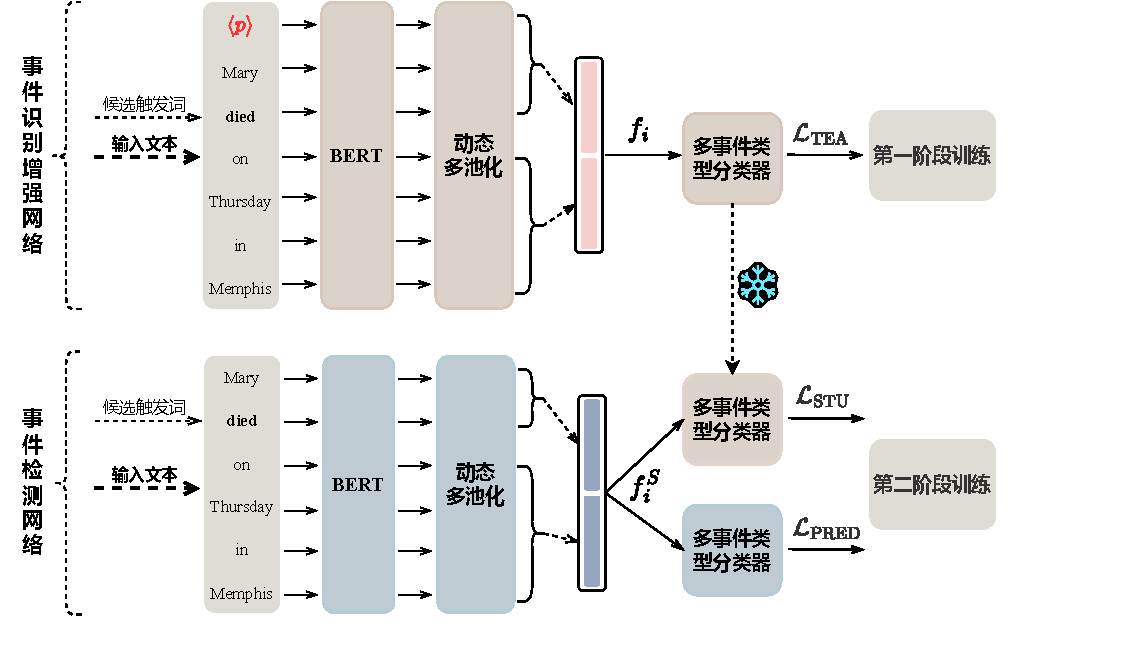
\includegraphics[width=1\linewidth]{figures/chap3/framework_cakd.pdf}
   \caption{基于DMBERT的CAKD方法架构图}
   \label{framework_cakd}
\end{figure}

\subsection{事件识别增强网络}

事件识别增强网络旨在在训练中引入句子级别识别信息,该信息可根据训练集的事件标签直接获取,不依赖于任何外部知识或资源。具体地,首先根据句子中是否存在事件触发词,将该句子标记为“\emph{Positive}”或“\emph{Negative}”。如果句子中不存在任何事件触发词,则该句子被标记为“\emph{Negative}”。如果至少存在一个事件触发词,则该句子被标记为“\emph{Positive}”。然后,基于在事件识别增强网络中使用的事件检测基线模型的类型,采用两种不同的方式在输入部分引入句子级别识别信息并进行相应编码,分别为:

\textbf{基于预训练词向量的事件检测模型}~对于句子中任意一个词$w_{i} \left(1 \leq i \leq n\right)$,首先拼接以下两类向量,表示为$\boldsymbol{x}_{i}$:
\begin{itemize}
    \item \textbf{原始输入向量}~采用其事件检测基线模型的原始输入设置。不同基线模型的输入向量有所差别,通常由预训练词向量、实体类型向量、词性标注向量和位置向量中的全部或部分串接得到。
    \item \textbf{句子级别识别向量}~通过随机初始化得到两个向量$\boldsymbol{s}_P$和$\boldsymbol{s}_N$,用于提供句子级别识别信息。若词$w_{i}$所在句子被标记为“\emph{Positive}”,则$w_{i}$对应的句子级别识别向量为$\boldsymbol{s}_P$,否则其对应的句子级别识别向量为$\boldsymbol{s}_N$。
\end{itemize}
然后,使用事件检测基线模型对输入$\boldsymbol{X}_\textrm{teacher} = (\boldsymbol{x}_{1}, \cdots, \boldsymbol{x}_{n})$进行编码。为了描述方便,本章选取Bi-LSTM~\cite{hochreiter1997long}作为基线模型,得到编码表示$\boldsymbol{f}_i \in {\mathbb{R}}^{d_{out}}$如下:
\begin{equation}
\label{eq3_1}
\boldsymbol{f}_i=\left[\overrightarrow{LSTM}\left(\boldsymbol{x}_{i}\right) ; \overleftarrow{LSTM}\left(\boldsymbol{x}_{i}\right)\right]
\end{equation} 

\textbf{基于预训练语言模型的事件检测模型}~对于句子中任意一个词$w_{i} \left(1 \leq i \leq n\right)$,首先根据句子级别识别信息在所在句子中插入可训练学习的特殊词元。具体地,若词$w_{i}$所在句子被标记为“\emph{Positive}”,则在句首插入特殊词元$\langle p \rangle$,否则在句首插入特殊词元$\langle n \rangle$。假设句首插入的特殊词元为$\langle p \rangle$,且选取DMBERT~\cite{wang2019adversarial}作为事件检测基线模型,则首先使用BERT~\cite{devlin2019bert}进行编码,得到特征表示如下:
\begin{equation}
  \left\{\boldsymbol{s}_P,\boldsymbol{h}_{1},\cdots,\boldsymbol{h}_{j},\cdots,\boldsymbol{h}_{n}\right\}=\textrm{BERT}(\langle p \rangle, w_{1},\cdots, w_{j},\cdots, w_{n})
\end{equation}
其中$\boldsymbol{s}_P$为$\langle p \rangle$对应的特征表示,$\boldsymbol{h}_{j} \left(1 \leq j \leq n\right)$为${w}_{j} \left(1 \leq j \leq n\right)$对应的特征表示。在此之后,使用一个动态多池化操作分段聚合编码后的特征表示:
\begin{equation}
    \left[\boldsymbol{h}_{1, i}\right]_{k}=\max \left\{\left[\boldsymbol{s}_P\right]_{k}, \left[\boldsymbol{h}_{1}\right]_{k} \cdots,\left[\boldsymbol{h}_{i}\right]_{k}\right\}
\end{equation}
\begin{equation}
    \left[\boldsymbol{{h}}_{i+1, n}\right]_{k}=\max \left\{\left[\boldsymbol{h}_{i+1}\right]_{k} \cdots,\left[\boldsymbol{h}_{n}\right]_{k}\right\}
\end{equation}
其中$[\cdot]_{k}$表示一个向量的第$k$个元素值。最后,串接上述表示得到$w_{i}$的特征表示$\boldsymbol{f}_i \in {\mathbb{R}}^{d_{out}}$:
\begin{equation}
\label{input_information}
\boldsymbol{f}_i=\left[\boldsymbol{h}_{1, i};\boldsymbol{{h}}_{i+1, n}\right]
\end{equation}

然后,对于不同类型的事件检测基线模型,将特征表示$\boldsymbol{f}_i$输入到多事件类别分类器,以计算概率分布$p\left(w_{i}\right)$如下:
\begin{equation}
  p\left(w_{i}\right) = \textrm{softmax}\left(\boldsymbol{W}_{S}\boldsymbol{f}_i + \boldsymbol{b}_{S}\right)
\end{equation}
其中$\boldsymbol{W}_{S} \in {\mathbb{R}}^{C \times d_{out}}$和$\boldsymbol{b}_{S} \in {\mathbb{R}}^{C}$表示分类器中需要学习训练的参数,其中$C$为预定义的事件类型数目。假设给定的批数据$\mathcal{B}$中存在$K$个词,其交叉熵损失$\mathcal{L_\textrm{TEA}}$计算如下:
\begin{equation}
  \mathcal{L_\textrm{TEA}} = -\sum^{K} \log p\left(e|w_{i}\right)
 \label{ce}
\end{equation}
其中$p\left(e|w_{i}\right)$表示事件识别增强网络将词$w_{i}$预测为正确的事件类型$e$的概率值。

\subsection{事件检测网络}

事件检测网络旨在建模事件检测任务,其使用原始的文本信息作为输入。然后,一方面基于固定的事件识别增强网络分类器参数设计辅助训练任务,引导事件检测网络自动从原始文本中捕获句子级别识别信息。同时,学习训练另一个分类器,以用于事件类型预测。

在事件检测网络输入部分,若使用基于预训练词向量的事件检测模型如Bi-LSTM进行编码,则移除$\boldsymbol{X}_\textrm{teacher} = (\boldsymbol{x}_{1}, \cdots, \boldsymbol{x}_{n})$中拼接的句子级别识别向量$\boldsymbol{s}_P$或$\boldsymbol{s}_N$,记作$\boldsymbol{X}_\textrm{student} = (\boldsymbol{x}_{1}^{S}, \cdots, \boldsymbol{x}_{n}^{S})$。然后,利用另一个Bi-LSTM~\cite{hochreiter1997long}得到编码表示$\boldsymbol{f}_i^{S} \in {\mathbb{R}}^{d_{out}}$如下:
\begin{equation}
\label{eq3_8}
\boldsymbol{f}_i^{S}=\left[\overrightarrow{LSTM}\left(\boldsymbol{x}_{i}^{S}\right) ; \overleftarrow{LSTM}\left(\boldsymbol{x}_{i}^{S}\right)\right]
\end{equation}

若使用基于预训练语言模型的事件检测模型如DMBERT,则首先利用另一个BERT编码不包含特殊词元$\langle p \rangle$或$\langle n \rangle$的原始文本:

\begin{equation}
  \left\{\boldsymbol{h}_{1}^{S},\cdots,\boldsymbol{h}_{j}^{S},\cdots,\boldsymbol{h}_{n}^{S}\right\}=\textrm{BERT}(w_{1},\cdots, w_{j},\cdots, w_{n})
\end{equation}
在此之后,同样使用一个动态多池化操作分段聚合编码后的特征表示,并进一步串接得到$\boldsymbol{f}_i^{S} \in {\mathbb{R}}^{d_{out}}$:
\begin{equation}
    \left[\boldsymbol{h}_{1, i}^{S}\right]_{k}=\max \left\{\left[\boldsymbol{h}_{1}^{S}\right]_{k} \cdots,\left[\boldsymbol{h}_{i}^{S}\right]_{k}\right\}
\end{equation}
\begin{equation}
    \left[\boldsymbol{{h}}_{i+1, n}^{S}\right]_{k}=\max \left\{\left[\boldsymbol{h}_{i+1}^{S}\right]_{k} \cdots,\left[\boldsymbol{h}_{n}^{S}\right]_{k}\right\}
\end{equation}
\begin{equation}
\label{input_information}
\boldsymbol{f}_i^{S}=\left[\boldsymbol{h}_{1, i}^{S};\boldsymbol{{h}}_{i+1, n}^{S}\right]
\end{equation}

然后,对于不同类型的事件检测基线模型,将特征表示$\boldsymbol{f}_i^{S}$输入到事件识别增强网络分类器中,计算概率分布$p^{S}\left(w_{i}\right)$如下:
\begin{equation}
  p^{S}\left(w_{i}\right) = \textrm{softmax}\left(\boldsymbol{W}_{S}\boldsymbol{f}_i^{S} + \boldsymbol{b}_{S}\right)
\end{equation}
给定包含$K$个词的批数据$\mathcal{B}$,其交叉熵损失$\mathcal{L_\textrm{STU}}$计算如下:
\begin{equation}
  \mathcal{L_\textrm{STU}} = -\sum^{K} \log p^{S}\left(e|w_{i}\right)
\end{equation}
其中$p^{S}\left(e|w_{i}\right)$表示将词$w_{i}$预测为正确的事件类型$e$的概率值。同时,将特征表示$\boldsymbol{f}_i^{S}$输入到另一个多事件类别分类器中,得到概率分布$p^{E}\left(w_{i}\right)$如下:
\begin{equation}
  p^{E}\left(w_{i}\right) = \textrm{softmax}\left(\boldsymbol{W}_{E}\boldsymbol{f}_i^{S} + \boldsymbol{b}_{E}\right)
\end{equation}
其中$\boldsymbol{W}_{E} \in {\mathbb{R}}^{C \times d_{out}}$和$\boldsymbol{b}_{E} \in {\mathbb{R}}^{C}$表示该分类器中需要训练的参数。给定包含$K$个词的批数据$\mathcal{B}$,则其交叉熵损失$\mathcal{L_\textrm{PRED}}$计算如下:
\begin{equation}
  \mathcal{L_\textrm{PRED}} = -\sum^{K} \log p^{E}\left(e|w_{i}\right)
 \label{ce}
\end{equation}
其中$p^{E}\left(e|w_{i}\right)$表示事件检测网络将词$w_{i}$预测为正确的事件类型$e$的概率值。

\subsection{训练和推理}
在训练阶段,首先基于损失$\mathcal{L_\textrm{TEA}}$训练事件识别增强网络。在完成事件识别增强网络训练后,固定其分类器参数$\boldsymbol{W}_{S}$和$\boldsymbol{b}_{S}$,并基于如下损失训练事件检测网络:
\begin{equation}
  \mathcal{L_\textrm{OVERALL}} = \mathcal{L_\textrm{STU}} + \mathcal{L_\textrm{PRED}}
  \label{overall_stu}
\end{equation}
其中最小化$\mathcal{L_\textrm{STU}}$能够在训练过程中通过共享固定的事件识别增强网络参数$\boldsymbol{W}_{S}$和$\boldsymbol{b}_{S}$,引导事件检测网络自动从文本中捕获句子级别识别信息。同时,最小化$\mathcal{L_\textrm{PRED}}$使得参数$\boldsymbol{W}_{E}$和$\boldsymbol{b}_{E}$聚焦于事件类型的分类建模。在推理阶段,使用$p^{E}\left(w_{i}\right)$获取$w_{i}$对应的事件类型。

\section{实验评估}

\subsection{实验设置}
\label{experiment_settings}
\textbf{1.数据集}~对于事件检测任务,本章使用了包含599个文档和33种事件类型的ACE2005语料库~\cite{doddington2004automatic},该语料库数据来源为报纸、新闻专线数据和广播新闻,由自动内容提取项目(Automatic Content Extraction,ACE)完成标注。其存在英文、中文和阿拉伯文版本,遵循最近的研究工作~\cite{chen2015event,lu2019distilling},本章使用英文版本(以下简称ACE2005数据集),并分别使用了529、40和30个文档作为训练集、验证集和测试集。此外,在训练集中,仅3325个句子存在至少一种事件,而剩余的10594个句子中不存在任何事件,因此其数据不平衡问题显著。

\textbf{2.评价指标}~本章实验遵循事件检测任务的标准评估~\cite{li2013joint,chen2015event}。如果事件触发词和对应的事件类型均与数据集标注的信息完全相同,则认定该事件触发词被正确检测,本章模型采用包括特殊事件类型$None$(空)的多分类方式同时识别事件触发词和预测对应的事件类型。
基于此,本章使用不区分事件类别的微平均方式计算准确率(P)、召回率(R)和F1值(F1)作为评估指标,具体如下:
\begin{equation}
   P=\frac{TP}{TP+FP}
\end{equation}
\begin{equation}
   R=\frac{TP}{TP+FN}
\end{equation}
\begin{equation}
   F1=\frac{2 \times P \times R}{P+R} 
\end{equation}
其中$TP$为检测出的正确事件触发词数目,$FP$为检测出的错误事件触发词数目,而$FN$则表示未被检测出的事件触发词数目。

\textbf{3.基线方法}~本节选择以下方法参与实验比较,这些方法均可基于不同的事件检测基线模型进行性能评估,具体包括:
\begin{itemize}
    \item \textbf{基线模型}:仅利用$\mathcal{L_\textrm{PRED}}$训练事件检测网络,其退化为对应的事件检测模型。
    \item \textbf{基线模型+Sim-CAKD}:本章提出的CAKD方法的简化版本。具体地,事件检测网络不额外学习训练新的多事件类别分类器,而直接利用事件识别增强网络的分类器进行事件类型的建模。因此,公式~\ref{overall_stu}中$\mathcal{L_\textrm{OVERALL}} = \mathcal{L_\textrm{STU}}$。在推理阶段,同样利用事件识别增强网络的分类器获取事件检测任务的结果。
    \item \textbf{基线模型+MTL}:遵循Ye等人~\cite{ye2019exploiting}消解关系抽取中数据不平衡依赖的思路,通过共享网络编码,增加额外的事件触发词识别任务,采用多任务学习方式进行建模。下文将介绍关键细节。
\end{itemize}

对于基线模型+MTL方法,假设给定句子中任意一个词$w_{i} \left(1 \leq i \leq n\right)$,根据选定的事件检测基线模型编码得到特征表示为$\boldsymbol{f}_i^{M}$。在事件触发词识别任务中,计算对应的二分类损失$\mathcal{L_\textrm{ID}}$如下:
\begin{equation}
  p^{I}\left(w_{i}\right) = \sigma\left(\boldsymbol{W}_{I}\boldsymbol{f}_i^{M} + \boldsymbol{b}_{I}\right)
\end{equation}
\begin{equation}
    \mathcal{L_\textrm{ID}} = - \sum^{K} \left(L_{i} \log p^{I}\left(w_{i}\right) + (1-L_{i}) \log \left(1-p^{I}\left(w_{i}\right)\right) \right)
\end{equation}
其中$\boldsymbol{W}_{I} \in {\mathbb{R}}^{1 \times d_{out}}$和$\boldsymbol{b}_{I} \in {\mathbb{R}}^{1}$分别表示该二分类器的训练参数,$\sigma(\cdot)$为sigmoid激活函数。当词$w_{i}$为事件触发词,则$L_{i}$设置为1,否则设置为0。而在事件检测任务中,将特征表示$\boldsymbol{f}_i^{M}$输入到多事件类别分类器中,得到对应的事件检测任务损失$\mathcal{L_\textrm{CL}}$:
\begin{equation}
  p^{C}\left(w_{i}\right) = \textrm{softmax}\left(\boldsymbol{W}_{C}\boldsymbol{f}_i^{M} + \boldsymbol{b}_{C}\right)
\end{equation}
\begin{equation}
  \mathcal{L_\textrm{CL}} = -\sum^{K} \log p^{C}\left(e|w_{i}\right)
 \label{ce}
\end{equation}
其中$\boldsymbol{W}_{C} \in {\mathbb{R}}^{C \times d_{out}}$和$\boldsymbol{b}_{C} \in {\mathbb{R}}^{C}$表示该分类器中需要训练的参数。基于损失$\mathcal{L_\textrm{ID}}$和$\mathcal{L}_\textrm{CL}$,则可得该多任务学习方法的总训练损失:
\begin{equation}    \mathcal{L}_\textrm{M}=\alpha\mathcal{L}_\textrm{ID}+(1-\alpha)\mathcal{L}_\textrm{CL}
\end{equation}
其中$\alpha$为权重超参数。

在本章所提的CAKD方法和上述基线方法中,不仅使用Bi-LSTM~\cite{hochreiter1997long},还利用以下事件检测基线模型参与性能验证:(1)Liu等人提出的JMEE~\cite{liu2018jointly},其融合了自注意力机制和GCN,以编码句法结构信息和捕捉不同事件间的关联。(2)Yan等人提出的MOGANED~\cite{yan2019event},其使用GAT网络聚合依存句法树中的多跳句法信息,以有效建模非邻接依存关系。(3)Wang等人提出的DMBERT~\cite{wang2019adversarial},其将DMCNN~\cite{chen2015event}模型中的CNN替换成BERT,并保留动态多池化操作。(4)本章提出的DMRoBERTa,其将DMBERT中的BERT替换成对应的改进版预训练语言模型RoBERTa~\cite{liu2019roberta},其他部分保持不变。

\textbf{4.实验配置}~对于基于预训练词向量的事件检测模型,各自原始输入向量保持不变,一般由预训练词向量、随机初始化的实体类型标签向量、位置向量和词性标注向量等组成,而其句子级别识别向量的维度均设置为300。此类事件检测模型的实验服务器配置均为:CPU型号Intel(R) Xeon(R) Gold 5218,主频2.30GHz;内存128G;GPU计算卡型号NVIDIA GeForce RTX 1080Ti,显存11G。对于基于预训练语言模型的事件检测模型,分别加载HuggingFace上发布的“google-bert/bert-base-uncased”文件\footnote{https://huggingface.co/google-bert/bert-base-uncased}和“FacebookAI/roberta-base”文件\footnote{https://huggingface.co/FacebookAI/roberta-base}作为编码使用的BERT和RoBERTa预训练模型参数。学习率均设置为5e-5,并使用AdamW进行训练优化。此类事件检测模型的实验服务器配置均为:CPU型号Intel(R) Xeon(R) Gold 5320,主频2.20GHz;内存256G;GPU计算卡型号NVIDIA GeForce RTX 3090,显存24G。此外,对于所有事件检测模型,其第一阶段训练均采用早停策略决定训练的轮次。当事件识别增强网络连续3轮在验证集上的F1指标没有出现提升,则结束该阶段的训练。在第二阶段训练中,若使用的基线模型为Bi-LSTM,则事件检测网络的轮次设置为30。对于其他事件检测基线模型,其事件检测网络采用对应事件检测模型的训练轮次或策略\footnote{DMRoBERTa参照DMBERT的训练轮次设置。}。本章实验均基于Pytorch~\cite{paszke2017automatic}框架完成。

\subsection{性能结果}
\label{3_3_2}

表\ref{tab:event}展示了在ACE2005数据集上的事件检测实验结果,其中$*$表示重新运行其发布的源代码得到的F1指标值。可以看出,本章所提的CAKD方法可以显著增强所有事件检测基线模型的F1指标,其涵盖了基于预训练词向量和预训练语言模型两种不同的类型。其中,CAKD方法能够大幅提升基于预训练语言模型的事件检测基线模型,分别在DMBERT和DMRoBERTa的F1指标上取得了4.0\%和3.8\%的性能提升。进一步,可以观察到对于所有的事件检测基线模型,CAKD方法在F1性能指标上都超过了相应的简化方法Sim-CAKD,其证明了将预测事件类型和学习句子级别识别信息的训练参数进行分隔,能提升对应基线模型的性能。对于MTL方法,其能够提升Bi-LSTM、DMBERT和DMRoBERTa等基线模型的F1性能表现,但其性能提升幅度均不如CAKD方法。而且,在使用了GNN网络架构的JMEE和MOGANED模型上,MTL方法降低了其对应的F1指标结果。因此,相比于MTL方法,本章所提的CAKD方法表现出在不同类型基线模型上的性能优势和通用性。此外,可以发现CAKD方法在不同基线模型上均主要通过显著增强预测的召回率提高整体的F1指标。该发现可以归因于本章提出的CAKD方法能够提升基线模型自动从文本中学习句子级别识别信息的能力,以更好地获取给定实例的正负实例情况,从而在事件检测中能以更高的置信水平预测出比例较小的正例数据。与之相反,基线模型本身在缺乏获取句子级别识别信息的能力时,倾向于避免将更多的给定实例预测为正例,导致较低的召回率。

\begin{table}[htp]
\centering
    \caption{ACE2005数据集上的事件检测性能结果}
	\begin{tabular}{lccc}
		\toprule
		模型 & P(\%) & R(\%) & F1(\%)  \\
		\midrule
		Bi-LSTM            & 68.6  & 67.0  & 67.8      \\
		Bi-LSTM+MTL            & 66.4  & 70.6  & 68.4        \\
		Bi-LSTM+Sim-CAKD   & 67.2  & 71.5  & 69.3      \\
        Bi-LSTM+CAKD   & 68.2  & 71.7  & \textbf{69.6}      \\
        \midrule
	 %    Bi-GRU            & 69.4  & 68.4  & 68.9      \\
		% Bi-GRU+MTL     & 67.0  & 73.3  & 70.0        \\
		% Bi-GRU+Sim-CAKD   & 67.5  & 73.8  & 70.5      \\
  %       Bi-GRU+CAKD   & 68.1  & 76.2  & \textbf{71.9}      \\
		% \midrule
		JMEE           & 75.3  & 70.5  & 72.8$^*$      \\
		JMEE+MTL            & 71.9  & 65.3  & 68.5      \\
		JMEE+Sim-CAKD           & 74.0  & 73.1  & 73.6      \\
        JMEE+CAKD           & 75.0  & 72.4  & \textbf{73.7}      \\
        	\midrule
		MOGANED          & 81.0  & 67.0  & 73.4$^*$      \\
		MOGANED+MTL            & 76.5  & 66.1  &  70.9     \\
		MOGANED+Sim-CAKD          & 79.4  & 69.1  & 73.9     \\
        MOGANED+CAKD           & 78.7  & 72.3  & \textbf{75.4}    \\
        	\midrule
		% EE-GCN          & 76.7   & 78.6  & 77.6      \\
		% EE-GCN+MTL            & 75.5  & 75.6  &  75.5     \\
		% EE-GCN+Sim-CAKD          & 76.2  & 79.1  & 77.6     \\
  %       EE-GCN+CAKD           & 76.4  & 79.9  & \textbf{78.1}    \\ \midrule
        DMBERT & 77.6 & 71.8 & 74.6   \\
	DMBERT+MTL &  75.3 & 77.7  & 76.5    \\
	DMBERT+Sim-CAKD & 76.0  & 81.2  & 78.5 \\
        DMBERT+CAKD & 75.6  & 81.9  & \textbf{78.6}  \\ \midrule
        DMRoBERTa & 71.1 & 80.5 & 75.5   \\
	DMRoBERTa+MTL & 76.4  & 76.0  &  76.2   \\
	DMRoBERTa+Sim-CAKD & 71.6  & 85.7  & 78.0 \\
        DMRoBERTa+CAKD & 73.7  & 85.9  & \textbf{79.3}  \\
		\bottomrule
	\end{tabular}
	\label{tab:event}
\end{table}

\subsection{与基于预训练语言模型的基线性能比较}

结合本章研究工作、DMBERT~\cite{wang2019adversarial}和RoBERTa~\cite{liu2019roberta}的发表时间,本章选取基于预训练语言模型且性能表现优秀的事件检测模型与CAKD方法作性能对比,具体包括:(1)Lai等人提出的GatedGCN~\cite{lai2020event},其基于BERT进行编码,并利用依存句法树在GCN中构建候选触发词特征表示对其他单词信息的过滤筛选。(2)Tong等人提出的EKD~\cite{tong2020improving},其基于BERT进行编码,并构建知识蒸馏框架,利用从WordNet获取的开放域触发词知识提升对训练集中稀疏和未出现事件触发词的识别。(3)Veyseh等人提出的GPTEDOT~\cite{veyseh2021unleash},其基于BERT进行编码,并利用GPT-2为事件检测生成额外的训练数据。此外,考虑到ChatGPT在多种自然语言处理任务上表现优异,Han等人~\cite{han2023information}利用情境学习(In-Context Learning,ICL)~\cite{brown2020language}构建5-shot ICL提示模版作为ChatGPT的输入,以生成ACE2005数据集上所有测试样本的事件检测结果。本章展示其F1指标作为性能参考。


表\ref{sota_comparison}展示的结果表明,DMRoBERTa+CAKD在F1指标上获得了最优性能,而DMBERT+CAKD也在F1指标上超越了GatedGCN和EKD模型。此结果表明,虽然只采用了简单的预训练语言模型编码和池化操作,但在应用了本章提出的CAKD方法后,与上述引入了外部知识资源如依存句法信息、WordNet和额外生成数据的事件检测模型相比,仍表现出具有竞争力的实验结果,进一步验证了CAKD方法的性能效率。另外,可以观察到ChatGPT的输入受限于少样本场景,在事件检测任务上性能表现不佳。

\begin{table}[htp]
\centering
    \caption{ACE2005数据集上基于预训练语言模型的事件检测性能结果对比}
	\begin{tabular}{lccc}
		\toprule
		模型 & P(\%) & R(\%) & F1(\%)  \\
		\midrule
        ChatGPT & - & - & 27.3 \\
        \midrule
		GatedGCN & 78.8 & 76.3 & 77.6       \\
		EKD & 79.1 & 78.0 & 78.6  \\ 
        GPTEDOT & 82.3 & 76.3 & 79.2 \\ \midrule  
        DMBERT+CAKD & 75.6  & 81.9  & 78.6  \\ 
        DMRoBERTa+CAKD & 73.7  & 85.9  & \textbf{79.3}  \\
		\bottomrule
	\end{tabular}
	\label{sota_comparison}
\end{table}

\subsection{事件触发词识别能力分析}

% 为了证明所提出的CAKD框架可以提高基线模型识别给定实例是正还是负例的能力(即事件触发词识别能力),
本节比较CAKD方法和相应的基线模型在事件触发词识别任务上的F1性能指标。如表\ref{tab:identification_compare}所示,在不同基线模型上引入CAKD方法,其识别事件触发词的性能均显著提升,证明其能够通用地消解数据不平衡依赖问题带来的正负例识别能力的下降。

\begin{table}[htp]
    \centering
    \caption{ACE2005数据集上的事件触发词识别任务F1(\%)指标结果}
	\begin{tabular}{lcc}
	    \toprule
		模型  & 基线模型  & 基线模型+CAKD   \\
		\midrule
		Bi-LSTM   & 70.1  & 71.6      \\
		JMEE      & 75.2  &  77.2        \\
		MOGANED   & 75.9  & 78.7    \\
            % EE-GCN   & 78.3  & 79.4    \\
            DMBERT   &  79.4 &  82.8   \\
            DMRoBERTa   &  80.1 &  84.3   \\   
		\bottomrule
	\end{tabular}
	\label{tab:identification_compare}
\end{table}

\subsection{数据不平衡程度分析}

本节分析在不同程度数据不平衡场景下,CAKD方法、MTL方法以及相应的基线模型方法在事件检测任务上的性能变化。具体地,在分析实验中采用DMRoBERTa作为基线模型,并依次从ACE2005数据集训练集中随机删减等间隔数量存在事件的句子数据,以构建存在不同数据不平衡程度的训练数据。如图\ref{imbalance}所示,随着数据不平衡程度的增加,不同方法的F1指标均呈现下降趋势,但DMRoBERTa+CAKD的下降最为平缓,在不同场景下的F1指标均显著优于同样应用了数据不平衡依赖消解的DMRoBERTa+MTL,验证了本章提出的CAKD方法在消解不同数据不平衡依赖的优势。进一步,可以观察到DMRoBERTa相比于应用了数据不平衡依赖消解的DMRoBERTa+CAKD和DMRoBERTa+MTL,在更加极端的不平衡数据场景下性能劣势显著增加,表明了数据不平衡依赖消解的必要性。

\begin{figure}[htp]
    \centering
   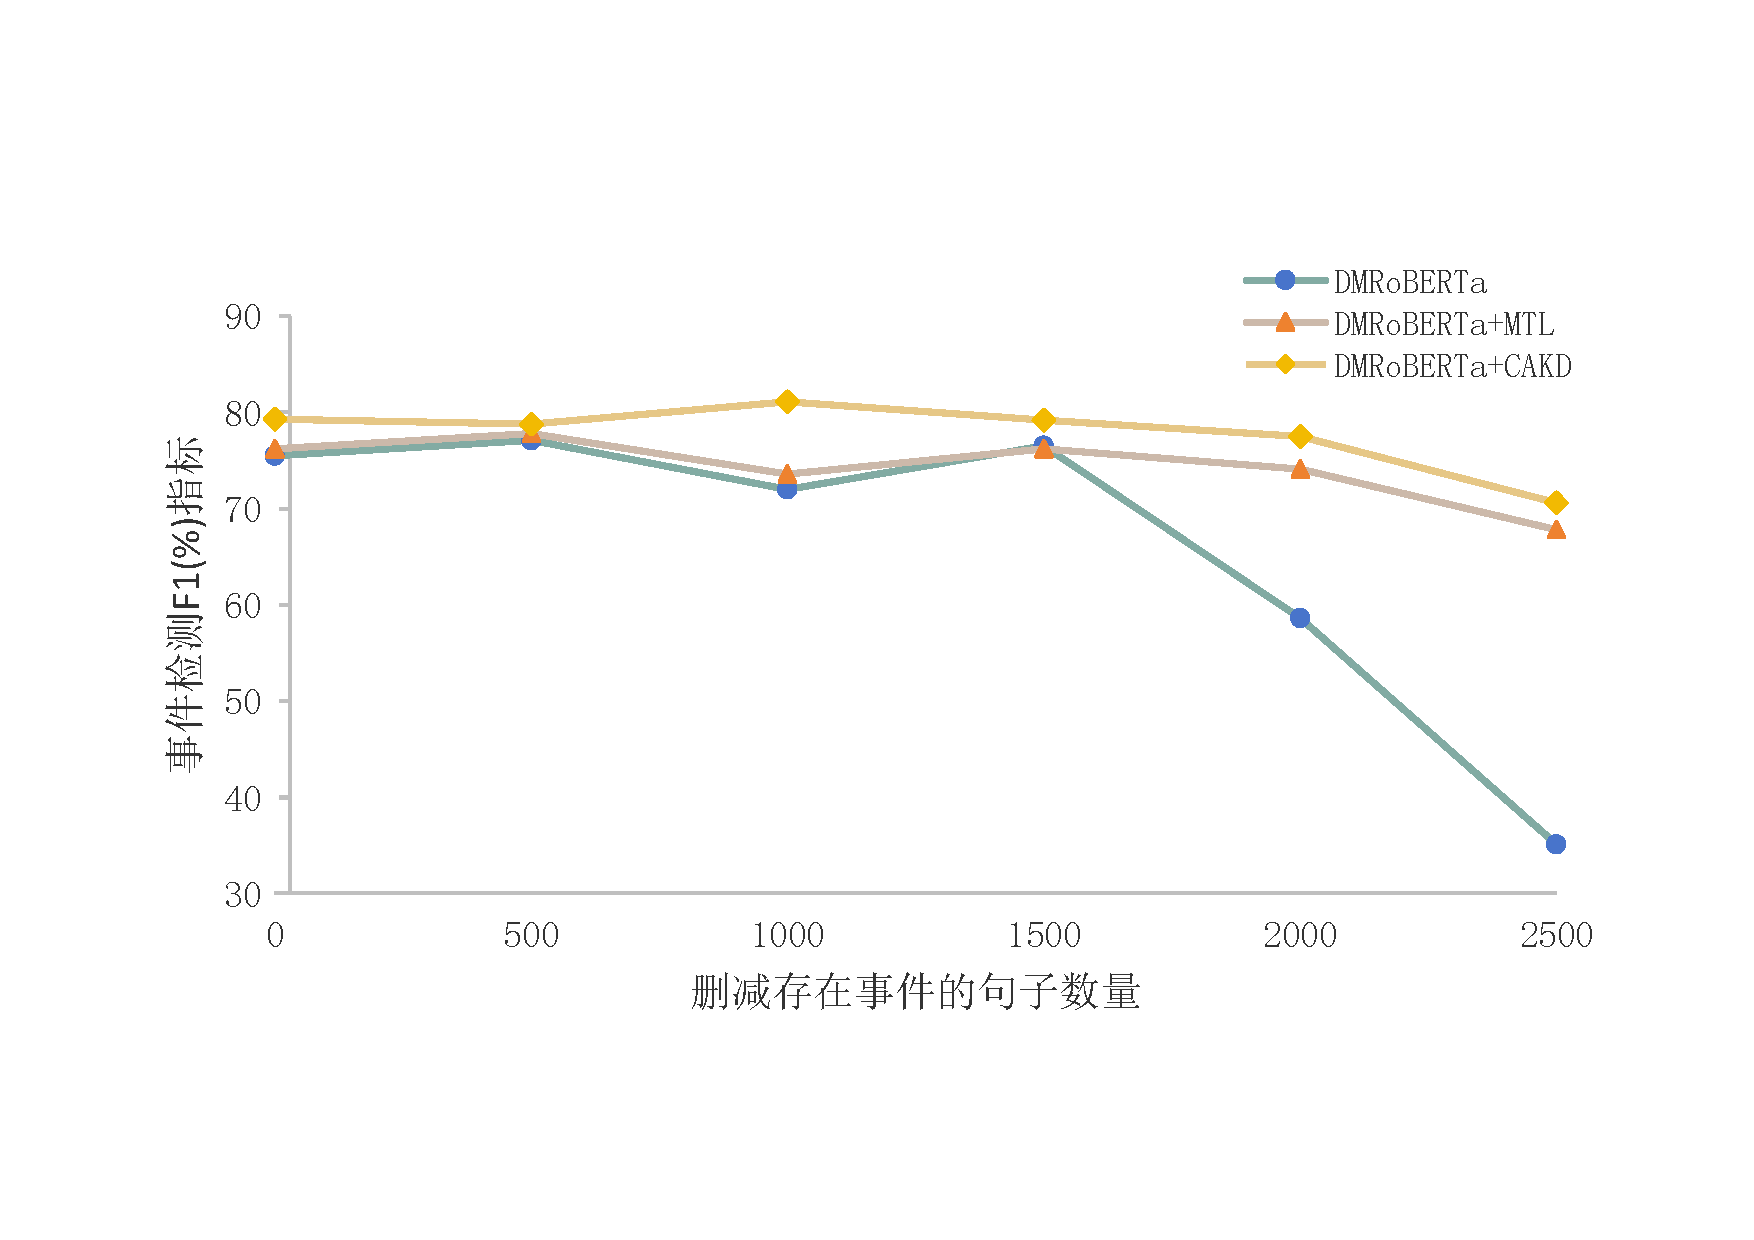
\includegraphics[width=0.8\linewidth]{figures/chap3/imbalance.pdf}
   \caption{不同程度数据不平衡下不同方法在F1(\%)指标上的结果对比}
   \label{imbalance}
\end{figure}

\subsection{案例研究}
本节基于ACE2005数据集中的具体实例进行案例分析。表\ref{case_study_event}展示了本章提出的CAKD方法和对应的基线模型在具体实例上的事件检测结果,其中粗体单词表示事件触发词,“频率”为对应事件类型的触发词占总事件触发词数目的比例。可以看到,在实例(1)中,虽然“acquitted”较为明显地触发了$Acquit$(宣判无罪)事件类型,基线模型仍由于该事件类型的稀疏性而将“acquitted”预测为非事件触发词。类似地,在实例(2)中,由于“rally”为罕见的事件触发词,基线模型无法识别出“rally”触发了$Demonstrate$(认定)事件类型。与之相比,CAKD方法能够基于文本内容建模句子级别识别信息,具备了更好地预测句子中是否存在事件的能力,相应提升了对于罕见事件类型和罕见事件触发词的识别,从而给出了正确的检测结果。

\begin{table*}[htp]
\centering
\small
\caption{ACE2005数据集上的案例分析}
\begin{tabular}{lcccc}
\toprule
\multicolumn{1}{c}{实例} & 正确事件标签 & 基线模型 & 基线模型+CAKD & 频率 \\ \midrule
\begin{tabular}[c]{@{}l@{}}(1) The Pakistani supreme court \\ last year \textbf{acquitted} Ayub Masih.\end{tabular} & Acquit & None & Acquit & 0.01\%  \\ \midrule
\begin{tabular}[c]{@{}l@{}}(2) Judge Shahid Rafiq..., found \\ Ranjha Masih guilty of defiling \\ Koranic verses during a protest \\ \textbf{rally} by the minority Christian \\ community in 1998.\end{tabular} & \multicolumn{1}{l}{Demonstrate} & None  & Demonstrate & 1.47\% \\ \bottomrule
\end{tabular}
\label{case_study_event}
\end{table*}

\subsection{其他信息抽取任务上的扩展实验}

为了进一步验证CAKD方法在其他任务上的良好扩展性,本章将CAKD方法迁移到信息抽取的另一关键任务—关系抽取上。在该任务中,数据不平衡问题同样严重存在。例如,在广泛使用的关系抽取数据集TACRED~\cite{zhang2017position}上,约80\%的实体对中不存在关系。因此,本章在TACRED数据集上比较CAKD方法和章节\ref{experiment_settings}中介绍的基线方法的性能结果。同样地,在这些方法中,使用不同的基线模型,包括Bi-LSTM、Bi-GRU、PA-LSTM~\cite{zhang2017position}、C-GCN~\cite{zhang2018graph}、C-AGGCN~\cite{guo2019attention}和GDPNet~\cite{xue2021gdpnet}。其中,在CAKD和Sim-CAKD方法中,采用和事件检测任务相似的策略,构建两个网络,在其中一个网络的输入中引入句子级别识别信息,并分别利用这些基线模型得到两个网络对应的编码表示,以替代公式\ref{eq3_1}和公式\ref{eq3_8}中的$\boldsymbol{f}_i$和$\boldsymbol{f}_i^{S}$,而方法中的其他部分则保持不变。

表\ref{relation_results}展示了在TACRED数据集上的关系抽取实验结果,其中$*$表示重新运行其发布的源代码得到的F1指标值。可以看出,将本章提出的CAKD方法迁移到不同的基线模型上,均提升了在关系抽取任务上的F1性能结果,有效地证明了本章所提方法的良好任务扩展性。同样地,其对应的简化方法Sim-CAKD也提升了不同关系抽取模型的整体性能,但其平均性能表现与CAKD方法存在一定差距,验证了与章节\ref{3_3_2}类似的结论,即分隔预测关系类型和学习句子级别识别信息的训练参数,能提升对应基线模型的性能。对于MTL方法,其能够提升Bi-LSTM和Bi-GRU模型的F1指标,但在其他关系抽取基线模型上表现不佳,进一步证明了该方法只适用于部分类型的网络架构模型。

\begin{table}[htp]
    \centering
    \caption{TACRED数据上的关系抽取性能结果}
	\begin{tabular}{lccc}
		\toprule
		模型 & P(\%) & R(\%) & F1(\%)  \\
		\midrule
		Bi-LSTM            & 65.7  & 58.9  & 62.1      \\
		Bi-LSTM+MTL            & 63.4  & 62.8  & 63.1       \\
        Bi-LSTM+Sim-CAKD            & 63.8  & 62.3  & 63.0    \\
		Bi-LSTM+CAKD   & 66.2  & 62.0  & \textbf{64.1}      \\
		\midrule
	    Bi-GRU            & 70.1 & 59.1  & 64.2      \\
		Bi-GRU+MTL     &  64.0 & 65.8  &  64.9       \\
		Bi-GRU+Sim-CAKD   &  66.7 & 64.5  &  65.6     \\
        Bi-GRU+CAKD   & 67.4 & 64.1  & \textbf{65.7}      \\
		\midrule
		PA-LSTM   & 65.7  & 64.5  & 65.1      \\
		PA-LSTM+MTL            & 66.2  & 63.4  & 64.8      \\
        PA-LSTM+Sim-CAKD            & 69.1  & 61.9  & 65.3        \\
		PA-LSTM+CAKD            & 67.1  & 66.4  & \textbf{66.7}     \\
		\midrule
		GCN            & 69.8  & 59.0  & 64.0      \\
		GCN+MTL            & 67.4  & 59.9  & 63.4      \\
		GCN+Sim-CAKD            & 68.1  & 62.5  & \textbf{65.2}        \\
        GCN+CAKD           & 68.5  & 61.7  & 64.9      \\
        \midrule
		C-GCN            & 69.9  & 63.3  & 66.4      \\
		C-GCN+MTL            & 69.8  & 62.2  & 65.8      \\
		C-GCN+Sim-CAKD            & 70.4  & 63.5  & 66.8        \\
        C-GCN+CAKD           & 69.7  & 65.0  & \textbf{67.3}      \\
        \midrule
		C-AGGCN            & 71.8  & 66.4  & 67.7$^*$      \\
		C-AGGCN+MTL            & 69.2  & 64.1  & 66.6      \\
		C-AGGCN+Sim-CAKD            & 71.6  & 64.7  & 68.0        \\
        C-AGGCN+CAKD           & 70.7  & 65.5  & \textbf{68.0}        \\
        \midrule
		GDPNet            & 72.0  & 69.0  & 70.5      \\
		GDPNet+MTL            & 69.9  & 66.9  & 68.4      \\
		GDPNet+Sim-CAKD            & 71.0  & 70.2  & 70.6        \\
        GDPNet+CAKD           & 71.3  & 70.6  & \textbf{70.9}        \\
		\bottomrule
	\end{tabular}
	\label{relation_results}
\end{table}

\section{本章小结}
本章首先研究了数据不平衡依赖对于事件检测性能的影响方式,并以此构建了句子级别识别信息进行辅助消解。进一步,本章提出了一种新的分类器自适应知识蒸馏的事件检测通用方法,其在事件识别增强网络输入部分通过学习的向量或特殊词元引入句子级别识别信息,并共享分类器参数引导事件检测网络自动捕捉该句子级别识别信息,实现事件检测的性能增强。本章在ACE2005数据集上使用不同事件检测基线模型进行了实验评估,评估结果表明本章提出的方法均能提升相应的性能结果。此外,本章通过实验验证了提出的方法能够自动适应不同数据不平衡程度和迁移到其他信息抽取任务上的能力,有效验证了提出的方法的多维度通用性。